\chapter{Phương pháp nghiên cứu}
\label{chap-Research_method}
\section{Định nghĩa bài toán}

\section{Kiến trúc hệ thống}

\section{Thu thập dữ liệu}\label{Research_data_crawl}
Hiện nay đa số  các sàn giao dịch lớn như Binance, Huobipro, OKCoin đều cung cấp api hỗ trợ cho phép xem lại các OrderBook, tỷ giá giao dịch các phiên trước đó, đặt lệnh giao dịch. Như đã đề cập ở chương 1, trong phạm vi sàn nghiên cứu của đề tài, chúng tôi chọn sàn Binance và các đồng cơ bản là BTC, ETH, USDT, BNB để nghiên cứu; Thông qua tìm hiểu, có hai thư viện hỗ trợ thu thập thông qua api trên sàn biannce là python-binance do sàn viết và ccxt (đã được Binance chứng nhận) đều được viết bằng ngôn ngữ python. Ccxt với khả năng hỗ trợ hơn 120 sàn khác nhau, hỗ trợ với nhiều ngôn ngữ lập trình, chính vì vậy ccxt được chọn làm thư viện chính để  thu thập dữ liệu và tạo các lệnh giao dịch để có thể mở rộng đề tài trong tương lai.\\
Để dễ hình dung về chức năng của api, api được ccxt chia thành hai loại là:
\begin{itemize}
    \item Public api: hỗ trợ lấy tickers, OrderBook; tỉ giá cặp tại thời điểm trước; các giao dịch trong khoảng thời gian trước đó.
    \item Private api: hỗ trợ tạo, hủy lệnh giao dịch; lấy các lệnh giao dịch trước đây; xem số đồng trong các ví của tài khoản sở hữu api này.
\end{itemize}
Quá trình chuẩn bị dữ liệu được thực hiện thông qua public api.\\
Khác với sàn giao dịch truyền thống (sàn chứng khoán), sàn giao dịch tiền mã hóa hoạt động liên tục vì vậy việc chia phiên giao dịch được sàn định nghĩa theo các khoảng thời gian cụ thể theo mặc định như 1 phút, 1 giờ, 1 ngày,... Điều này giúp cho người tham gia có thể biết tỷ giá trong các phiên giao dịch trước. Tuy nhiên trong phiên giao dịch có thể gồm nhiều các giao dịch với giá, số lượng đồng khác nhau. Nhằm dễ  thống kê, public api cung cấp để lấy giá OHLCV( Open, High, Low, Close, Volume) tương ứng với giá mở sàn; giá cao nhất, thấp nhất trong phiên; giá đóng sàn và lượng đồng trao đổi. Đây là các đặc trưng cơ bản cho một phiên giao dịch. Dữ liệu sẽ được lưu dạng bảng với mỗi dòng tương ứng với một phiên giao dịch gồm thời gian mở phiên theo dạng Unix time, và 5 đặc trưng nêu trên, các đặc trưng khác sẽ được trình bày tóm tắt như sau:
\begin{itemize}
    \item Tổng số giao dịch mua; bán.
    \item Số lượng đồng mua; bán trung bình
    \item Độ lệch chuẩn số lượng đồng mua; bán.
    \item Giá trung bình của các  giao dịch mua; bán và độ lệch chuẩn tương ứng.
    % \item Tổng số lượng mua; bán
\end{itemize}
Trong trường hợp một phiên giao dịch không có giao dịch mua nào bán hoặc không có giao dịch bán, tổng giao dịch sẽ bằng 1 và các trường trung bình, độ lệch chuẩn sẽ là 0. Trong thực nghiệm, hiếm khi xảy ra trường hợp này, cụ thể với khoảng thời gian từ 2017/08/17 đến 2019/09/01 có 16 phiên giao dịch như trên trong tổng số  17875 phiên giao dịch với khoảng thời gian phiên là 1 giờ cho cặp BTC/USDT.

\section{Tiền xử lý dữ liệu}
Sau công đoạn thu thập dữ liệu thô từ sàn, các phiên giao dịch được vectơ hóa và sắp xếp theo thời gian thành bảng được lưu dạng csv. Bước tiền xử lý dùng dữ liệu trên với các bước được tóm tắt theo hình sau:
\begin{figure}[H]
% TODO thêm  combine --> d-diff --> REMOVE
	\center	\includegraphics[width=1.0\textwidth]{./figures/Preprocessing_data.png}
	\caption{Tiền xử lý dữ liệu}
	\label{fig:Preprocessing_data}

\end{figure}

% Data Cleaning: Data is cleansed through processes such as filling in missing values, smoothing the noisy data, or resolving the inconsistencies in the data.
% Data Integration: Data with different representations are put together and conflicts within the data are resolved.
% Data Transformation: Data is normalized, aggregated and generalized.
% Data Reduction: This step aims to present a reduced representation of the data in a data warehouse.
% Data Discretization: Involves the reduction of a number of values of a continuous attribute by dividing the range of attribute intervals.

\subsection{Thêm đặc trưng}
Ngoài các đặc trưng được lấy trực tiếp từ sàn, Trong một phiên giao dịch với các giá High, Low chênh lệch nhau không rõ rệt khi thời gian phiên ngắn như 1 phút, 1 giờ; cần chọn thêm các đặc trưng như giá chênh lệch giữa High-Low và giá chênh lệch giữa Close-Open sẽ hiệu quả, đặc biệt khi chuẩn hóa z-score, min-max; hệ số chuẩn hóa được tăng lên giúp tăng độ lệch chuẩn đối với đặc trưng mới này khi so sánh các phiên giao dịch với nhau.
\subsection{Sai phân bậc d}
Khi sử dụng sai phân bậc d,
Sử dụng 1d order difference, thể hiện sự chênh lệch giá hiện tại với giá trước.

% https://www.kaggle.com/reisel/how-to-handle-correlated-features
\subsection{Lựa chọn đặc trưng}
Dữ liệu sau khi được thêm các đặc trưng mới, các đặc trưng có các mức tương đồng khác nhau, việc lựa chọn đặc trưng là điều cần thiết để loại bớt các đặc trưng tương quan với nhau. 
% TODO moving average:

\subsection{Chuẩn hóa dữ liệu}

% Normalize
Với dữ liệu dạng bảng mỗi dòng tương ứng một phiên giao dịch, các dòng được sắp xếp với thời gian tăng dần. Tập dữ liệu được chia thành tập huấn luyện và tập kiểm thử.  Khi chuẩn hóa dữ liệu tập huấn luyện tạo ra hệ số chuẩn hóa, hệ số này sẽ chuẩn hóa tập dữ liệu kiểm thử với giả thiết khi có tập huấn luyện, một giao dịch mới sẽ được chuẩn hóa theo hệ số trước đây. Điều này có hạn chế  khi chuẩn hóa theo min-max với khoảng $[0, 1]$ hoặc $[-1, 1]$ giá trị của các giao dịch trong tập kiểm thử có thể vượt ngoài 1, để tránh trường hợp này có thể  xóa các dữ liệu bất thường này hoặc dùng phép chuẩn hóa khác như \textit{z}-score:\\
\begin{align}
  Z_{scale} = \frac{Z - \mu}{\sigma},  
\end{align}
trong đó:
\begin{itemize}
    \item $Z$ là giá trị trước khi chuẩn hóa.
    
    % TODO: độ lệch chuẩn hiệu chỉnh
    \item $\mu$, $\sigma$ lần lượt là giá trị trung bình, độ lệch chuẩn trước khi hiệu chỉnh.
    
    \item $Z_{scale}$ là giá trị sau khi chuẩn hóa.
    
\end{itemize}

\section{Đánh nhãn dữ liệu} \label{data-labeling}
Nhãn được chia thành hai loại là xu hướng tăng và xu hướng giảm của giá đóng phiên thời điểm hiện tại. Thống kê với dữ liệu BTC/USDT thời gian 1 giờ có 9051 nhãn xu hướng tăng và 8452 nhãn xu hướng giảm, trường hợp giá không đổi tại phiên giao dịch sau là không có. Công việc đánh nhãn được thực hiện sau khi gộp các phiên giao dịch thành các điểm dữ liệu như hình sau:
\begin{figure}[hbt!]
% 	\center	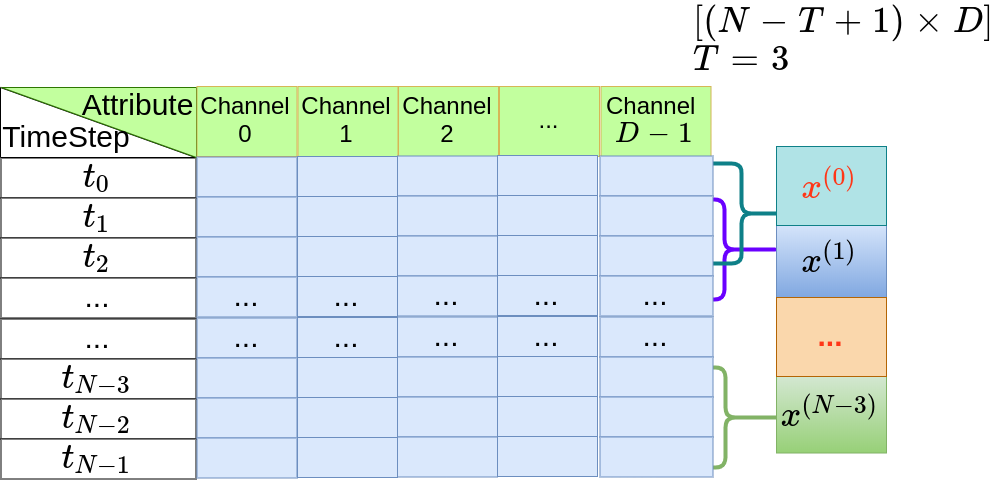
\includegraphics[width=1.0\textwidth]{labeling.png}
    \centering
	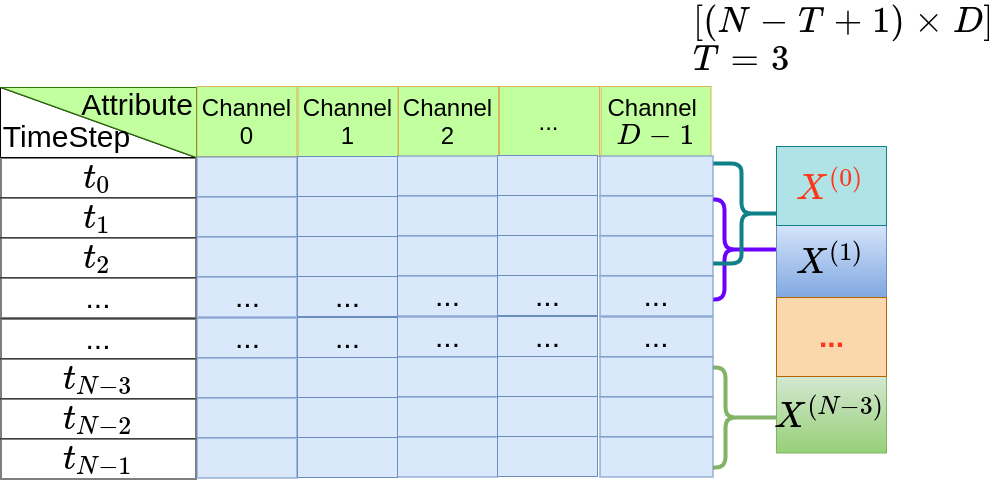
\includegraphics[width=.8\textwidth]{figures/labeling.png}
	\caption{Đánh nhãn dữ liệu}
	\label{fig:Labeling}

\end{figure}


Với các tham số:
\begin{itemize}
    \item $D$: Số thuộc tính của mỗi phiên giao dịch
    \item $T$: Số phiên giao dịch liên tiếp (Sliding window)
\end{itemize}


\subsection*{Các điểm hạn chế của ba mô hình nêu trên}
Trong ba mô hình kể trên có điểm chung là mỗi điểm dữ liệu được đưa vào trong quá trình huấn luyện là thông tin của một phiên giao dịch. Tuy nhiên với dữ liệu theo dạng thời gian thực, mỗi điểm dữ liệu cần chứa các thông tin phiên giao dịch hiện tại cũng như các phiên giao dịch trước đó. Để biểu diễn mối quan hệ giữa các phiên giao dịch liên tục nhau trên điểm dữ liệu, ta có thể thêm các thuộc tính mới như giá trị trung bình của 5 phiên giao dịch trước, độ chênh lệch của giá mở, giá đóng phiên. Tuy nhiên bước xử lý dữ liệu trước khi đưa vào chứa các tham số cố định. Một hướng làm khác khi gộp nhiều phiên giao dịch liên tục nhau thành một điểm dữ liệu dẫn tới bùng nổ số  chiều dữ liệu. Vấn đề này dẫn chúng tôi tới ý tưởng thu giảm số chiều và `học' tự động dữ liệu thông qua các bộ lọc (filters) thay cho bước tiền xử lý dữ liệu. Thông qua tìm hiểu, nhóm đã tham khảo thêm mô hình variational autoencoder. Chi tiết mô hình sẽ được trình bày tại phần tiếp theo.

\subsection{Mô hình Variational autoencoder}
Để giải thích mô hình Variational Auto Encoder, chúng tôi nêu ý tưởng của mô hình Auto Encoder, sau đó đi đến khái niệm mô hình Variational Auto Encoder và cách ứng dụng để làm công đoạn phân loại.
\subsection{Mô hình Autoencoder}
Kiến trúc của mô hình Auto Encoder gồm 2 mô-đun chính là Encoder, Decoder. Với ý tưởng chính là `nén' xuống chiều không gian nhỏ hơn. Trên chiều không gian mới này (latent space), dữ liệu được thu giảm từ không gian phức tạp thành các phần đơn giản hơn (simple components). Để đảm bảo hơn cho quá trình nén ít bị mất thông tin (nói cách khác trên chiều không gian nhỏ có thể khôi phục lại dữ liệu gốc) ta cần lớp giải nén (Decoder) với nhiệm vụ giải nén về dữ liệu ban đầu. Khi dữ liệu đi ra từ Encoder được giải nén qua Decoder trùng khớp với dữ liệu ban đầu, ta có thể hiểu rằng số  bậc tự do (degrees of freedom) nhỏ hơn so với số chiều của dữ liệu gốc. Việc phân cụm dữ liệu trở nên rõ ràng hơn trên chiều mới và điều này được thí nghiệm trên nhiều loại dữ liệu ảnh\cite{autoencoder-for-molecular-design}.
\subsection{Mô hình Variational autoencoder}
Mô hình Variational autoencoder (VAE) sử dụng trong đề tài là một biến thể khác của mô hình Autoencoder với ràng buộc rằng biến ẩn được sinh theo một hàm phối tiên nghiệm (prior distribution). Việc dự đoán có đầu vào là biến ẩn được lấy mẫu (sampling) từ đầu ra của mạng Encoder. Kiến trúc của mô hình sử dụng được mô tả theo Hình \ref{fig:VAE-arch}.
\begin{figure}[H]
	\center	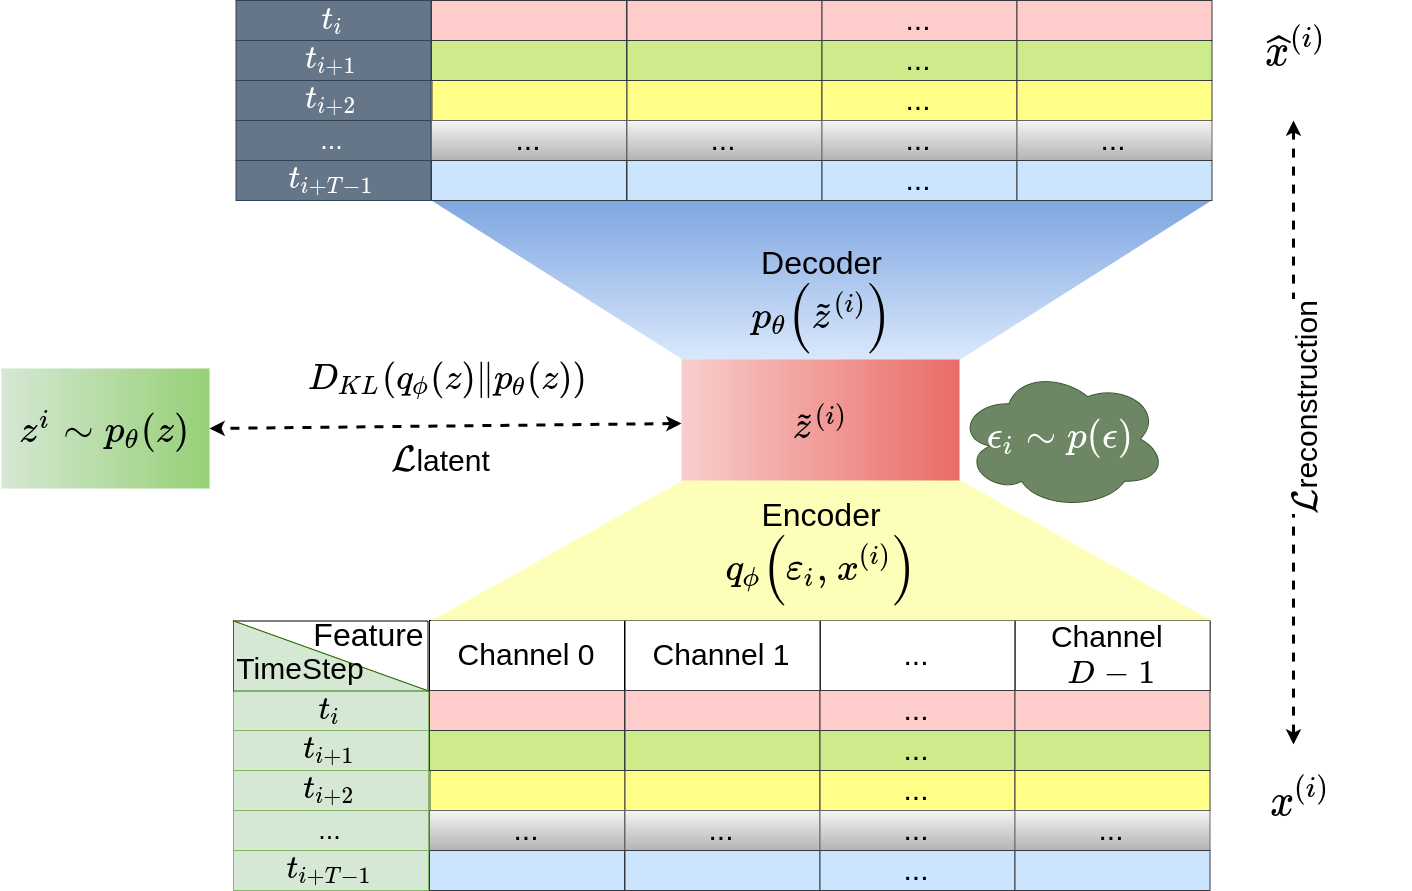
\includegraphics[width=1.0\textwidth]{figures/VAE/pngs/VAE_Arch.png}
	\caption{Kiến trúc mô hình dựa trên Variational Auto Encoder}
	\label{fig:VAE-arch}
\end{figure}

Để chi tiết hơn mô hình, chúng tôi sử dụng các kí hiệu cho các giả thiết sau:
\begin{itemize}
    \item $X = \{x^{(i)}\}_{i=1}^N$ gồm $N$ các điểm dữ liệu có phân phối đồng nhất độc lập (iid).
    \item Giá trị $z^{(i)}$ được sinh ra từ phân phối tiên nghiệm $p_{\theta^*}(z)$.
    \item Giá trị $x^{(i)}$ được sinh ra từ phân phối đồng thời $p_{\theta^*}(x \given z)$.
\end{itemize}

 Mục tiêu của bài toán là việc dự đoán cần phải chính xác đồng thời mô hình tìm được phân phối của dữ liệu đã cho theo phân phối tiên nghiệm. Trong phần thực nghiệm, chúng tôi có sử dụng mạng nơ-ron cho từng mô-đun vì lý do dễ dàng cập nhật trọng số  khi có được hàm lỗi.
 
 \textbf{Hàm lỗi cho việc phân loại:} $\mathcal{L}_C$ dựa được tính theo lỗi của hàm softmax.
 \textbf{Hàm lỗi cho việc tối đa likelihood theo phân phối tiên nghiệm:}
\begin{align}
  \mathcal{L}_{MLE} = -\frac{1}{N} \sum_{i=1}^N log(p_\theta(x^{(i)}))  
\end{align}

Với mô-đun Encoder, Decoder và Classifier là hàm tất định, tuy nhiên vì lý do $z$ được sinh mẫu ngẫu nhiên nên không thể xây dựng hàm lỗi một cách trực tiếp vì lý do khi khai triển $p_\theta(x)$:
\begin{equation} \label{eq:intractable_likelihood}
p_\theta(x) = \int p_\theta(z)p_\theta(x \given z) dz
\end{equation}
với :
\begin{itemize}
    \item $p_\theta(z)$ là phân phối tiên nghiệm có thể tính được.
    \item $p_\theta(x \given z)$ là phân phối có thể tính được thông qua mô-đun Decoder.
\end{itemize}

Tuy nhiên không thể tính được (intractable) cho toàn bộ $z$ trên miền liên tục. Khi khai triển phân phối hậu nghiệm: $p_\theta(z \given x)$ đưa về dạng không thể phân giải được do $p_\theta(x)$:
\begin{align}
  p_\theta(z \given x) = \frac{p_\theta(x \given z)p_\theta(z)}{p_\theta(x)}\label{eqn:intractable_posterior}.
\end{align}
Một cách giải quyết vấn đề trên là xấp xỉ hàm lỗi theo phương pháp suy luận biến phân được trình bày kĩ hơn tại Tiểu mục \ref{variational-lower-bound}. Theo phương pháp này khi khai triển $\log p_\theta(x)$:
\begin{align}
\log p_\theta(x^{(i)})  \geq \mathcal{L}(x^{(i)}, \theta, \phi) 
\end{align}
Với:

\begin{align}
\mathcal{L}(x^{(i)}, \theta, \phi) = \mathbb{E}_{z} \left[\log p_\theta(x^{(i)} \given z) \right]
    - \mathbb{E}_{z} \left[\log \frac{q_\phi(z \given x^{(i)})}{p_\theta(z)} \right]
\label{eq:elbo_loss}
\end{align}



Việc tối ưu $p_\theta(x^{(i)})$ thay bằng việc tối ưu cận dưới $\mathcal{L}(x^{(i)}, \theta, \phi)$. Lúc này hàm lỗi mới thay cho hàm $\mathcal{L}_{MLE}$ được tính như sau:
\begin{align}
  \mathcal{L}_{ELBO} &= -\frac{1}{N} \sum_{i=1}^N 
  \left(
  \mathbb{E}_{z} \left[\log p_\theta(x^{(i)} \given z) \right]
    - \mathbb{E}_{z} \left[\log \frac{q_\phi(z \given x^{(i)})}{p_\theta(z)} \right]
  \right)\\
  &= \mathcal{L}_{reconstruction} + \mathcal{L}_{latent}
\end{align}

Trở lại với kiến trúc VAE, phương trình  \eqref{eq:elbo_loss} 
có thể mô tả như sau:
\begin{itemize}
    \item $\mathbb{E}_{z} \left[\log p_\theta(x^{(i)} \given z) \right]$ : được tính theo mô-đun Decoder khi tái tạo lại $x$ từ $z$.
    \item $\Dkl{q_\phi(z \given x^{(i)})}{p_\theta(z)}$: Kullback–Leibler divergence giữa hai phân phối hậu nghiệm và tiên nghiệm.
\end{itemize}


\begin{subequations}\label{eq:sub}
	\noeqref{eq:1,eq:2}
	\begin{gather}
	\frac{\text{d}b_1}{\text{d}z} - \beta_1b_1 = C_{12}b_2,\label{eq:1}\\
	\frac{\text{d}b_2}{\text{d}z} - \beta_2b_2 = C_{21}b_1.\label{eq:2}
	\end{gather}
\end{subequations}
\eqref{eq:sub}


% Khi giá trị của hàm $\mathcal{L}_{ELBO}$ được giảm trong quá trình huấn luyện. Hai lỗi $$
Hai hàm lỗi được trực quan theo Hình \ref{fig:VAE-describe} dưới đây:
%%%%%%%%%%%%%%%%%%% Figure VAE loss describe
\begin{figure}[H]
	\center	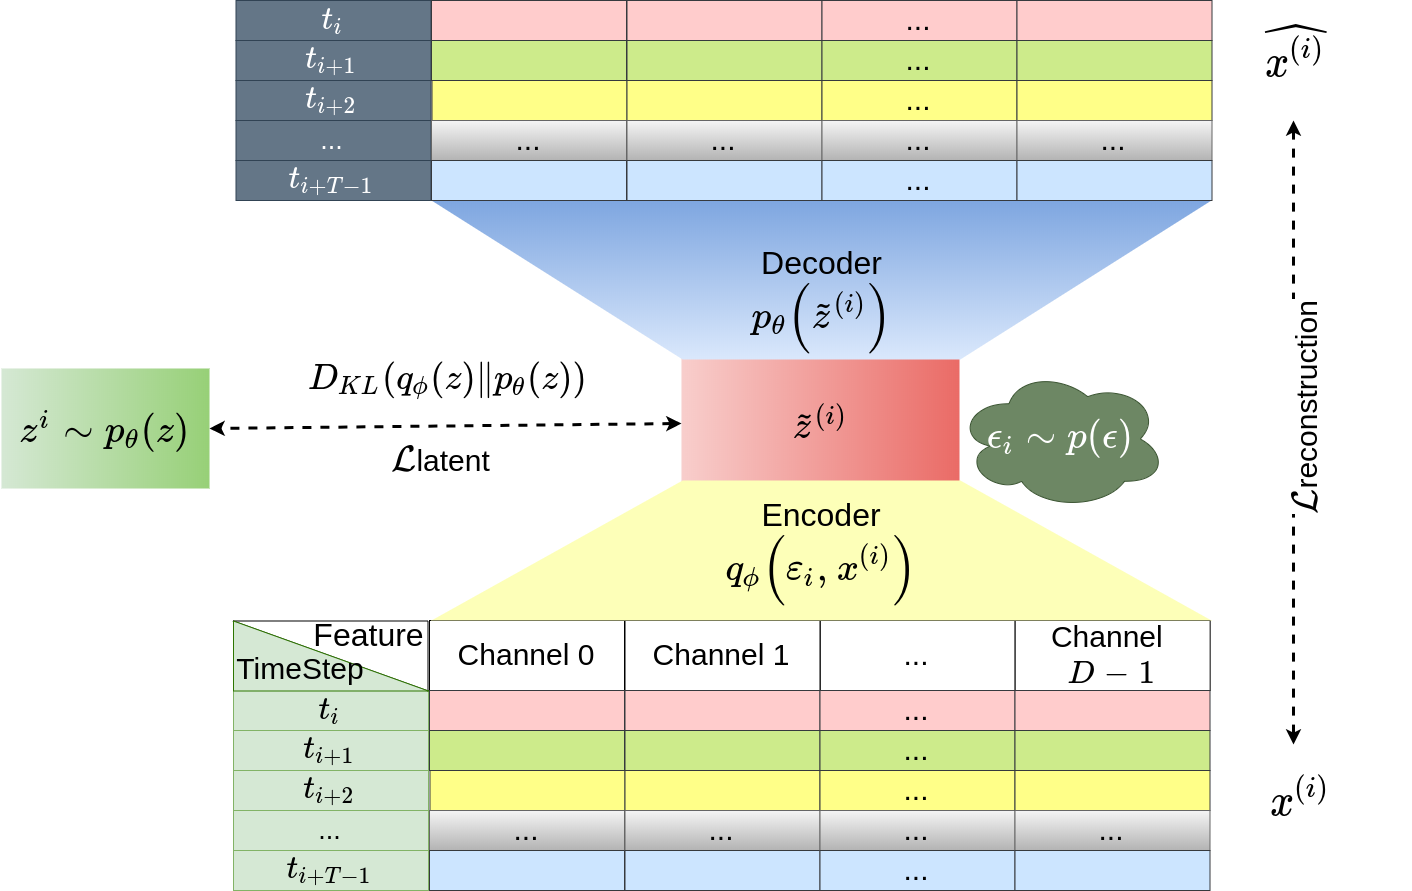
\includegraphics[width=1.0\textwidth]{figures/VAE/pngs/VAE_Arch_Describe.png}
	\caption{Mô tả hàm lỗi trong mô hình VAE}
	\label{fig:VAE-describe}
\end{figure}

Mục tiêu của bài toán là giảm được giá trị của hàm $\mathcal{L}_{ELBO}$. 
Trong trường hợp hội tụ cần đảm bảo phân phối hậu nghiệm $q_\phi(z \given x^{(i)})$ có các tham số từ mô-đun Encoder được tiến về phân phối tiên nghiệm cho trước: $p_\theta(z)$, đồng thời với phân phối hậu nghiệm có thể tái tạo lại dữ liệu cho trước. Nói cách khác, từ quá trình huấn luyện, mô hình có thể `học' được phân phối dữ liệu ban đầu từ phân phối tiên nghiệm đơn giản hơn được cho trước.

Trong phần hiện thực, chúng tôi có giả định biến ẩn (latent variable) có số chiều là $n_z$ thuộc phân phối multivariate normal distribution với vector trung bình là $\mu = 0 \in \mathbb{R}^{n_z}$, và hiệp phương sai là $\Sigma = I \in \mathbb{S}_{++}^{n_z}$. Theo đó, $ \mathcal{L}_{latent}$ được tính như sau:
\begin{align}
     \mathcal{L}_{latent} &= \Dkl{q_\phi(z \given x^{(i)})}{\mathcal{N}(0, I)}\\
     &= \frac{1}{2}\sum_{i=1}^{n_z}(\sigma_i^2 + \mu_i^2 - \log(\sigma_i^2) -1) \geq 0
\end{align}
Với dữ liệu thời gian, việc tính lỗi $\mathcal{L}_{reconstruction}$ không thể chuyển (scale) dữ liệu về khoảng $[0-1]$ vì trong phiên tiếp theo, các biến có giá trị vượt ngoài phạm vi $[0-1]$. Cụ thể, với 1 tháng trước tỷ giá trong phạm vi từ 2000 đến 5000, khi đưa dữ liệu tháng sau có tỷ giá là 5500 vượt ngoài khoảng trên. Vì lý do trên, chúng tôi lựa chọn hàm log mean square error để thể hiện lỗi khi tái tạo lại dữ liệu:
\begin{align}
     \mathcal{L}_{reconstruction} &= \frac{1}{N}\sum_{i=1}^N \log((x^{(i)} - \hat{x}^{(i)})^2) \geq 0
\end{align}

\begin{figure}[H]
	\center	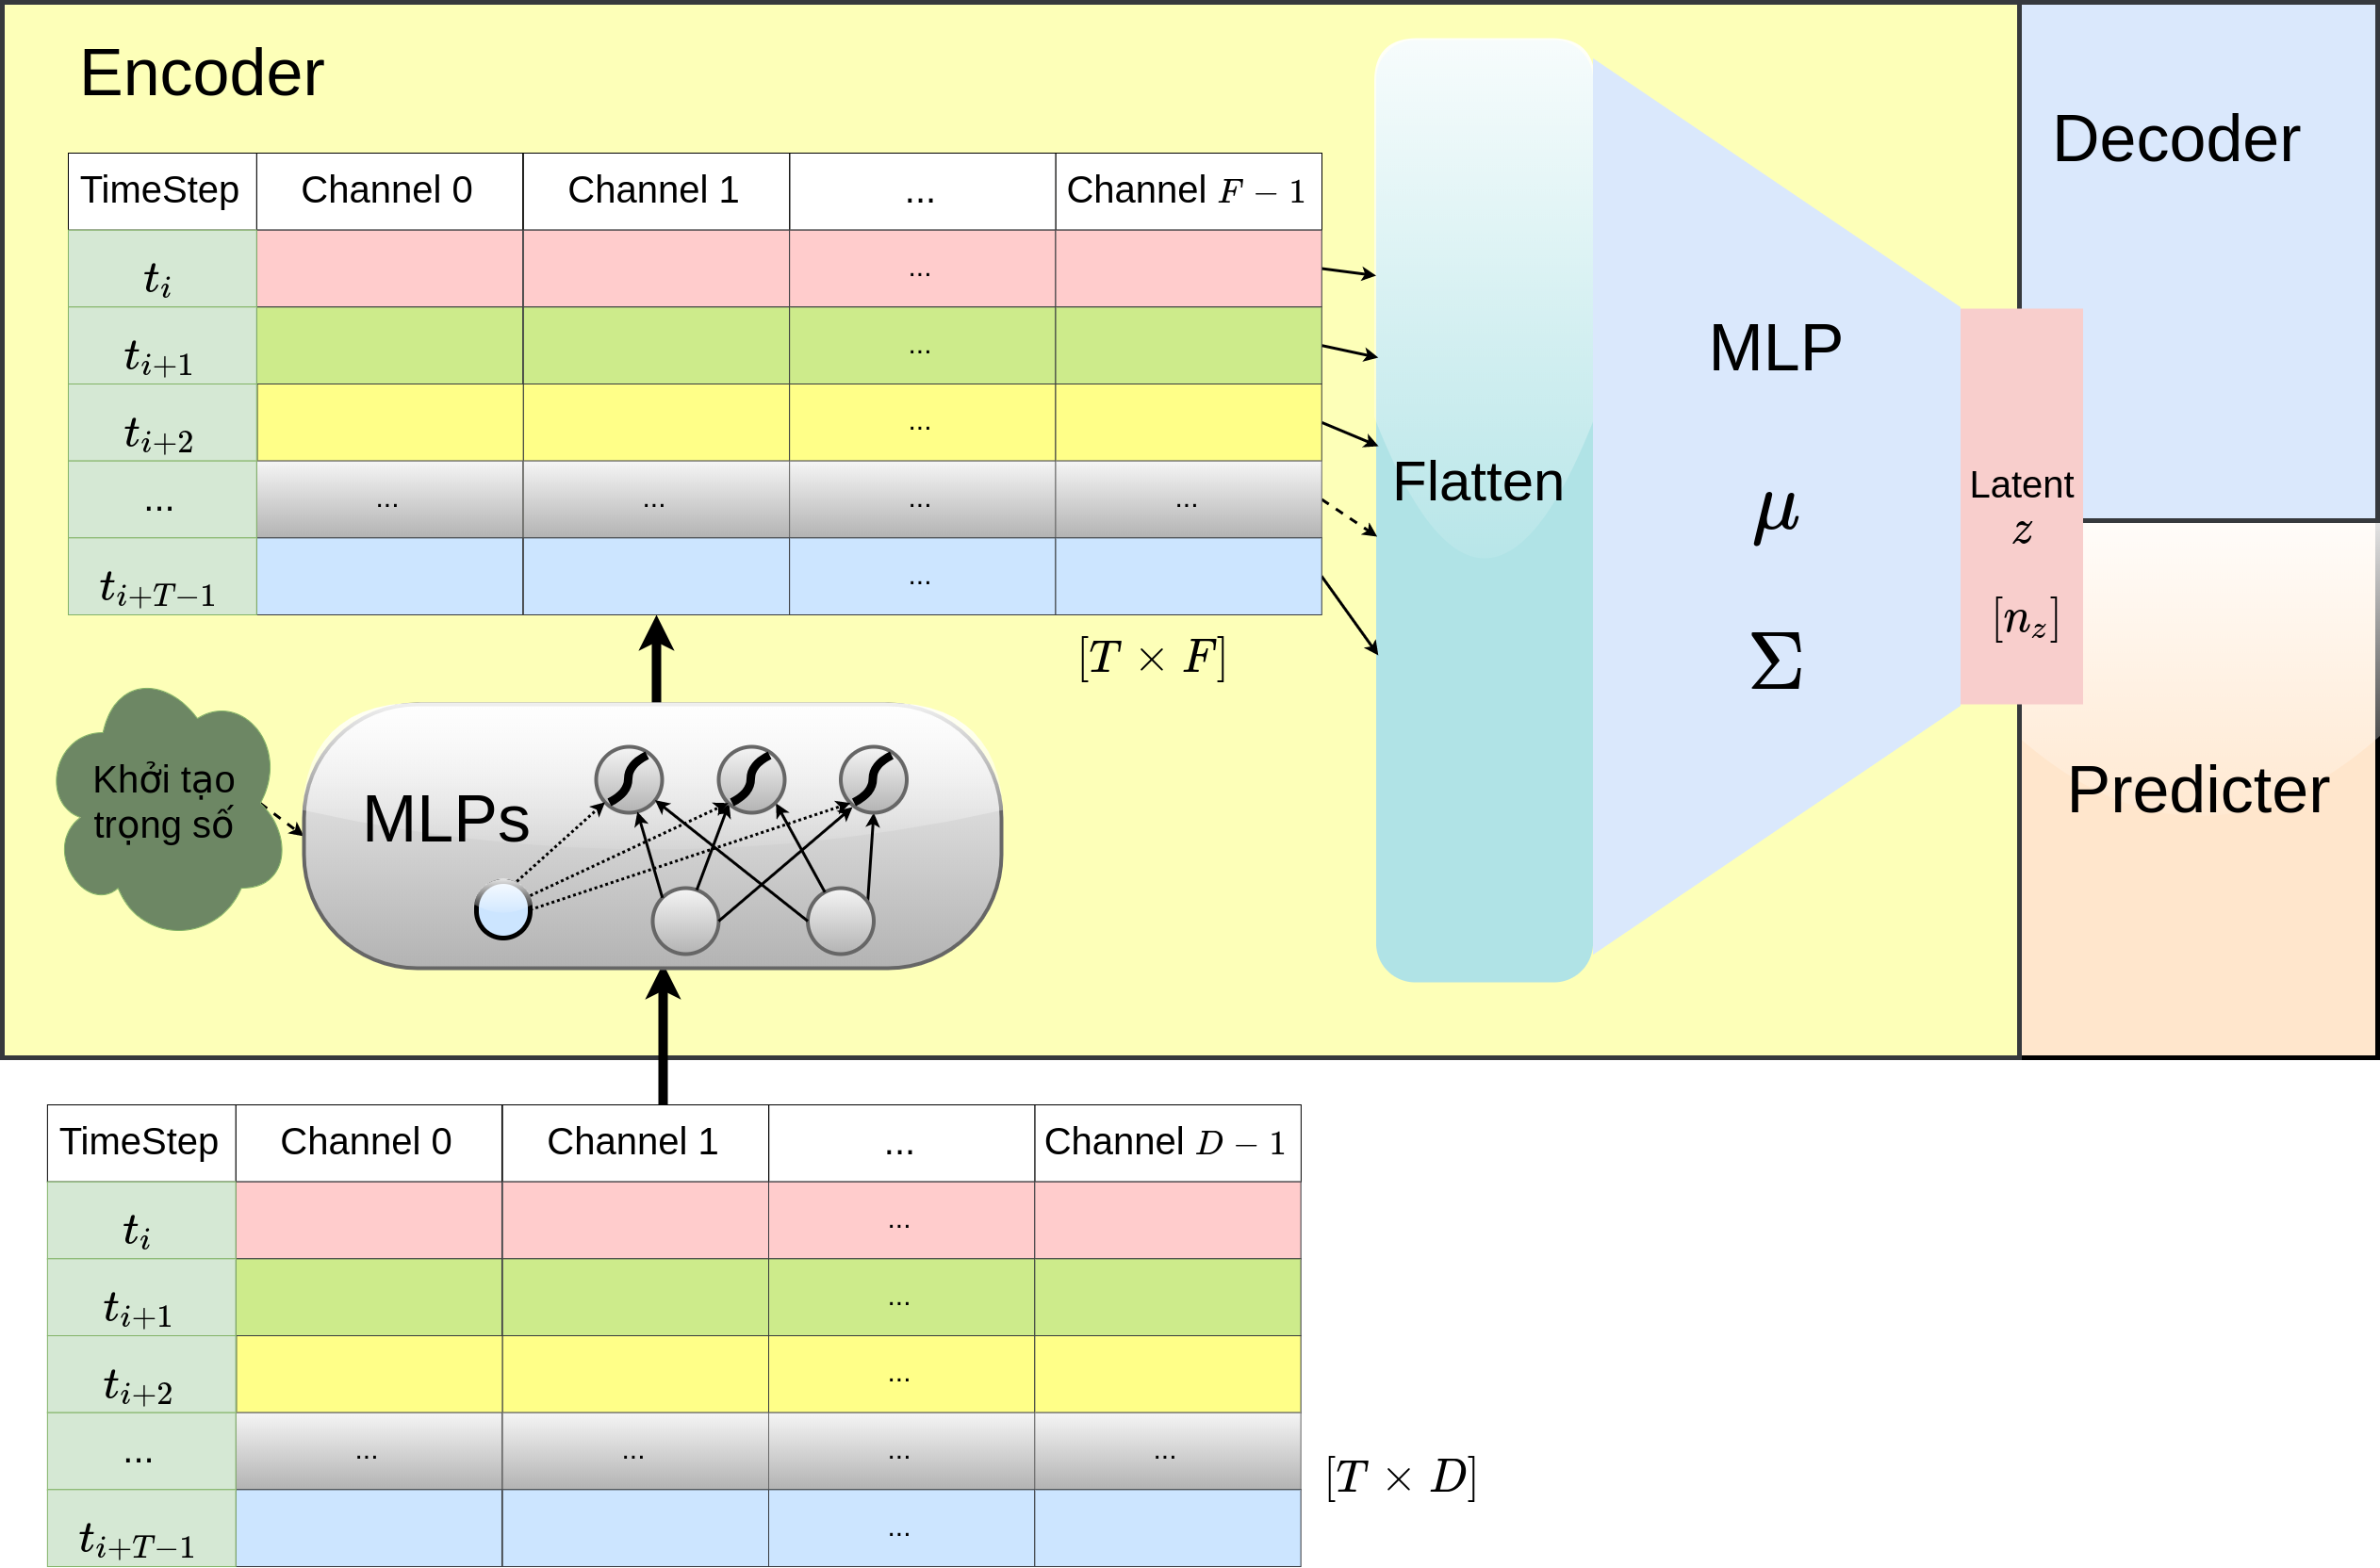
\includegraphics[width=1.0\textwidth]{figures/VAE/pngs/VAE_Encoder.png}
	\caption{Kiến trúc mô-đun Encoder}
	\label{fig:VAE-encoder}

\end{figure}